\chapter{Material-system reproduction (capstone)}
\label{ch:p10}

\begin{keybox}
\textbf{Key idea.} This is the ``put it all together on a real system''
capstone. You pick ONE documented blend from the materials database, load
\emph{every} parameter through the validated loader (never hand-copied),
reproduce a published morphology trend, and then \emph{stress} that
conclusion --- mesh convergence, time convergence, and a parameter-uncertainty
sweep --- so you can state honestly which conclusions are ROBUST and which are
artefacts of the tutorial scale.
\end{keybox}

\begin{keybox}
\textbf{Learning objectives.} Load a real material with its full provenance and
audit which numbers are measured, fitted, or assumed; reproduce a
rate-dependent morphology trend on the de-confounded matched-dryness axis;
run mesh and time convergence on a production system; propagate an
order-of-magnitude parameter uncertainty; and separate robust physics from
tutorial-scale noise.\\[2pt]
\textbf{Prerequisites.} Chapter~\ref{ch:p5} (the drying film and matched
terminal state), Chapter~\ref{ch:p4} (ternary Flory--Huggins), and
Chapter~00 (environment green).\\[2pt]
\textbf{Expected cost.} Quick mode $<2$~min (a two-rung smoke on a $16\times16$
mesh); reference mode a few to $\sim$20~min ($\PtenNrungs$-rung ladder plus one
finer mesh, two time steps, and two chi values on a $32\times32$ mesh);
research mode a $64\times64$ ladder with a $128\times128$ convergence rung.
\end{keybox}

\section{The system and its provenance}

We reproduce a trend for \textbf{\PtenSystem}, a diketopyrrolopyrrole
donor blended with a PCBM-class acceptor and spin-coated from chloroform,
after the drying study of Negi et~al.\ (recorded in \file{materials.yaml}).
It is the natural choice here because it carries a concrete Flory
interaction triple, concrete degrees of polymerization, AND an explicit
spin-speed $\rightarrow$ Biot ladder --- literally ``the real chi, $N$, and
Biot.'' Every parameter is loaded through \file{materials/loader.py}; the run
archives the resolved values and their provenance to
\file{materials.resolved.json}.

The capstone is built around an honest audit: which of these numbers can you
trust? The loader exposes each parameter's \emph{status}, \emph{source}, and
\emph{uncertainty}. For \PtenSystem\ every parameter is
\PtenProvStatus\ / fitted --- \emph{representative} values, NOT measured table
entries --- and the polymer--fullerene interaction $\chi_{pf}=\PtenChiPF$
carries an \emph{order-of-magnitude} uncertainty of $\PtenChiPFunc$.
Fig.~\ref{fig:p10prov} is that audit, generated directly from the loaded
provenance.

% --- generated by gen_figures.py ---
\begin{figure}[h]\centering
  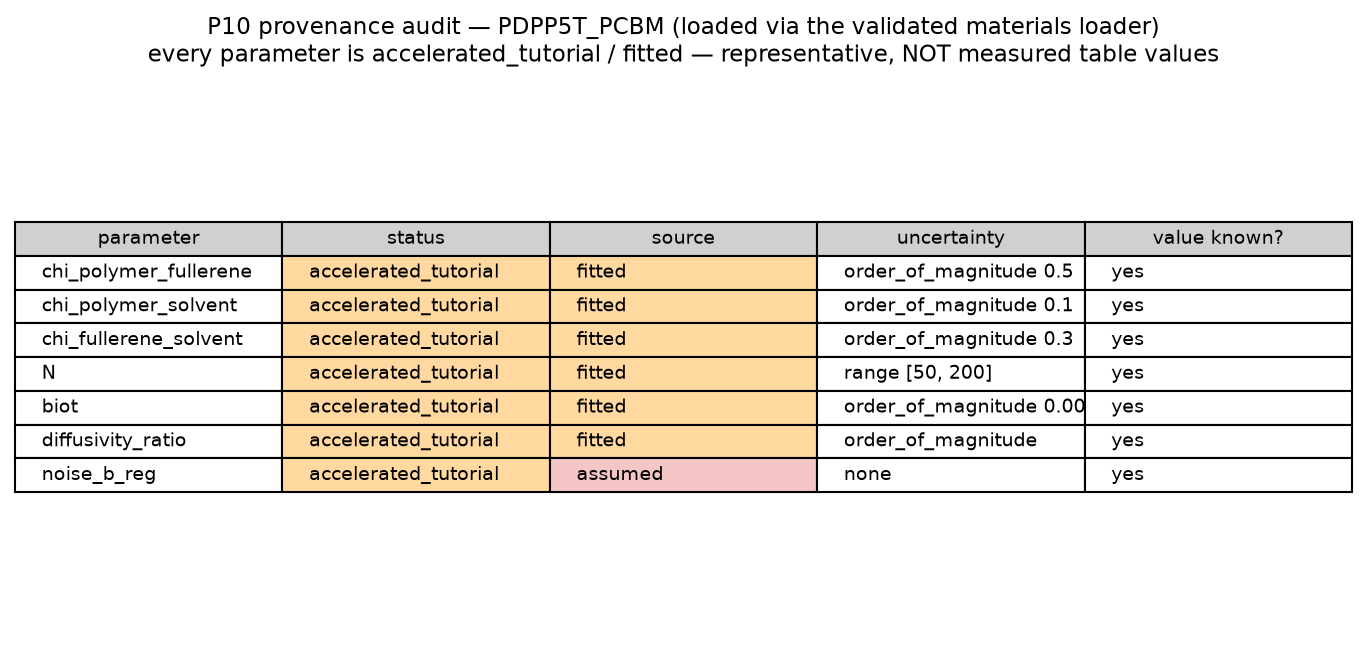
\includegraphics[width=\linewidth]{figures/p10_provenance.png}
  \caption{Provenance audit of every loaded \PtenSystem\ parameter: status
  (production vs.\ accelerated-tutorial), source type (measured / fitted /
  assumed), uncertainty, and whether the value is even known. This governs how
  much weight any downstream conclusion can bear.}
  \label{fig:p10prov}
\end{figure}

\paragraph{An honest negative on the archetype.} The archetypal
organic-solar-cell blend P3HT:PCBM is the more famous evaporation-morphology
benchmark, but at its recorded weak $\chi_{pf}\approx0.86$ with a large polymer
$N$ it barely demixes at tutorial scale (almost no lateral contrast within the
horizon). We document that as a genuine finding and choose \PtenSystem, which
demixes robustly, so the trend study has signal to measure.

\section{The reproduced trend}

Negi et~al.\ vary the \emph{spin speed}, which sets the drying \emph{rate}:
higher rpm removes solvent faster. Evaporation is the clock of morphology
formation (Chapter~\ref{ch:p5}): faster drying gives the blend less time to
phase-separate before it is quenched, so the classical expectation is a
\emph{finer} frozen morphology at higher rpm. The database records the spin
speed as a Biot ladder $\mathrm{Bi}(\text{rpm})$.

\paragraph{Reproducing only what is reproducible.} Two facts about those
recorded Biot numbers govern how we use them, and both are honoured in the run
provenance. First, their absolute magnitudes are illustrative and carry an
order-of-magnitude uncertainty, so neither the absolute Biot nor even the exact
ratio between rungs is meaningful --- only the \emph{ordering} (higher rpm $=$
faster drying) is. Second, as recorded they are $\sim\!10^{-3}$, far too small
to dry a film within the tutorial horizon. We therefore reproduce the
physically robust content --- the monotone spin-speed $\rightarrow$ drying-rate
ordering --- by mapping the $\PtenNrungs$ recorded rungs, in rank order, onto a
moderate, resolvable drying-rate window in $k_e$ (the Chapter~\ref{ch:p5}
drying regime, $\mathrm{Bi}\in[\PtenBiSlow,\PtenBiFast]$). Morphology is then
read at MATCHED dryness --- the same mean solvent fraction $\phi_s$ for every
rung --- so drying RATE is never confounded with final STATE.

\begin{runbox}
\textbf{Run it.}
\begin{lstlisting}
cd physics/10_material_case_study
python run_harness.py --config configs/p10.yaml --mode reference \
    --output outputs/p10 --overwrite
python gen_figures.py --run-dir outputs/p10   # figures + numbers
\end{lstlisting}
The harness loads \PtenSystem\ through the validated loader, marches the
$\PtenNrungs$-rung drying ladder, reads morphology at matched dryness, runs the
mesh + time convergence and the $\chi_{pf}$ sensitivity sweep, and gates
\file{results.json} against \file{baseline.yaml}.
\end{runbox}

% --- generated by gen_figures.py ---
\begin{figure}[h]\centering
  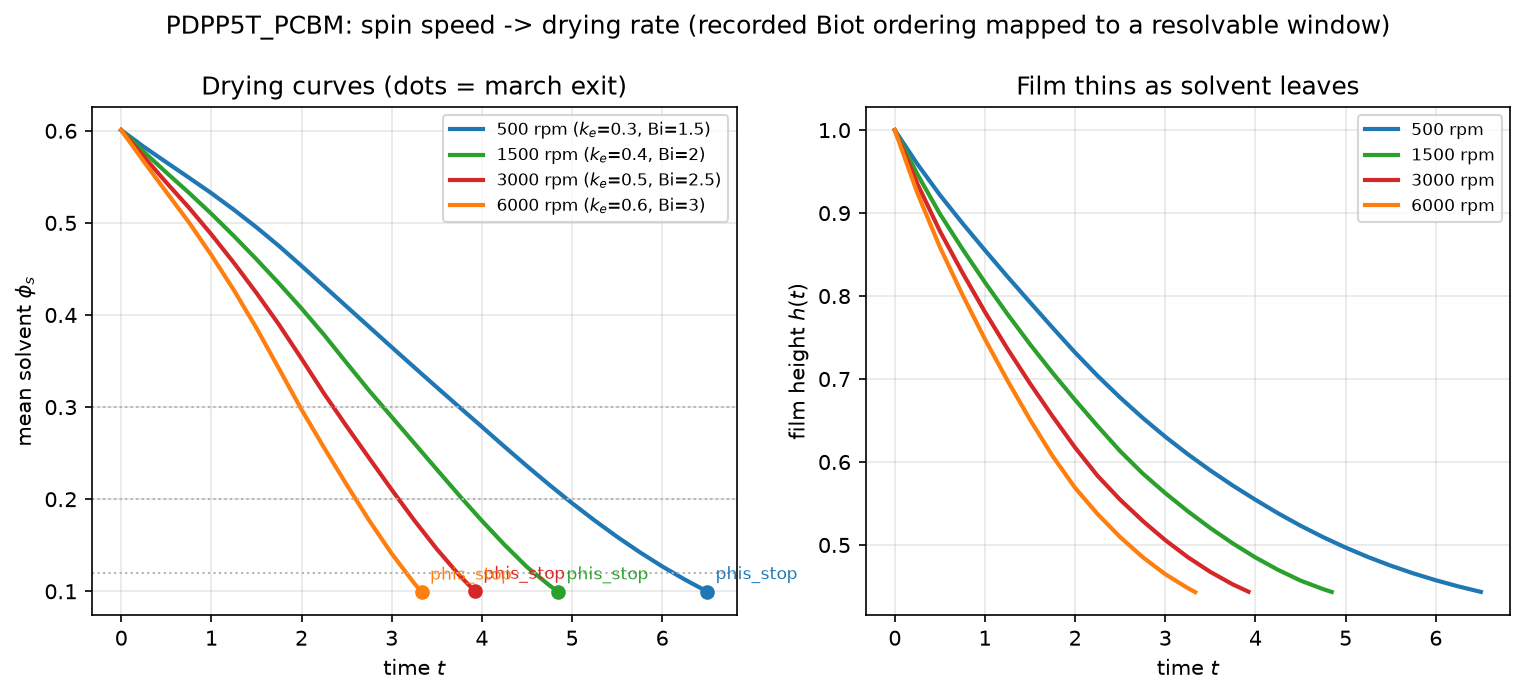
\includegraphics[width=\linewidth]{figures/p10_ladder.png}
  \caption{Drying curves $\phi_s(t)$ and film height $h(t)$ for the spin-speed
  ladder. Every rung is driven past the smallest matched dryness (dotted
  lines); dots mark the march exit, so a truncated run is never mistaken for a
  dried one.}
  \label{fig:p10ladder}
\end{figure}

\paragraph{What you should see.} At matched dryness the ``faster $=$ finer''
wavelength ordering is \emph{weak and noisy} at tutorial scale (single seed,
only a few lateral domains): the slowest rung ($\PtenSlowRpm$~rpm) and fastest
rung ($\PtenFastRpm$~rpm) give matched-$\phi_s$ wavelengths of $\PtenWLslowMid$
and $\PtenWLfastMid$ cells, and whether the faster film is strictly finer comes
out as ``\PtenFinerOrder.'' What \emph{is} robust is visible in
Fig.~\ref{fig:p10matched}: the DEGREE of demixing --- the phase contrast ---
is set by DRYNESS. It rises monotonically as the film dries (contrast
$\PtenContrastSlowHi \rightarrow \PtenContrastSlowMid \rightarrow
\PtenContrastSlowLo$ from wet to dry on the slow rung) and is nearly
rate-independent at matched dryness (spread $\PtenContrastRateSpread\%$ across
the whole ladder). The matched-state wavelength collapses onto the Biot number
to within $\PtenBiCollapseSpread\%$.

% --- generated by gen_figures.py ---
\begin{figure}[h]\centering
  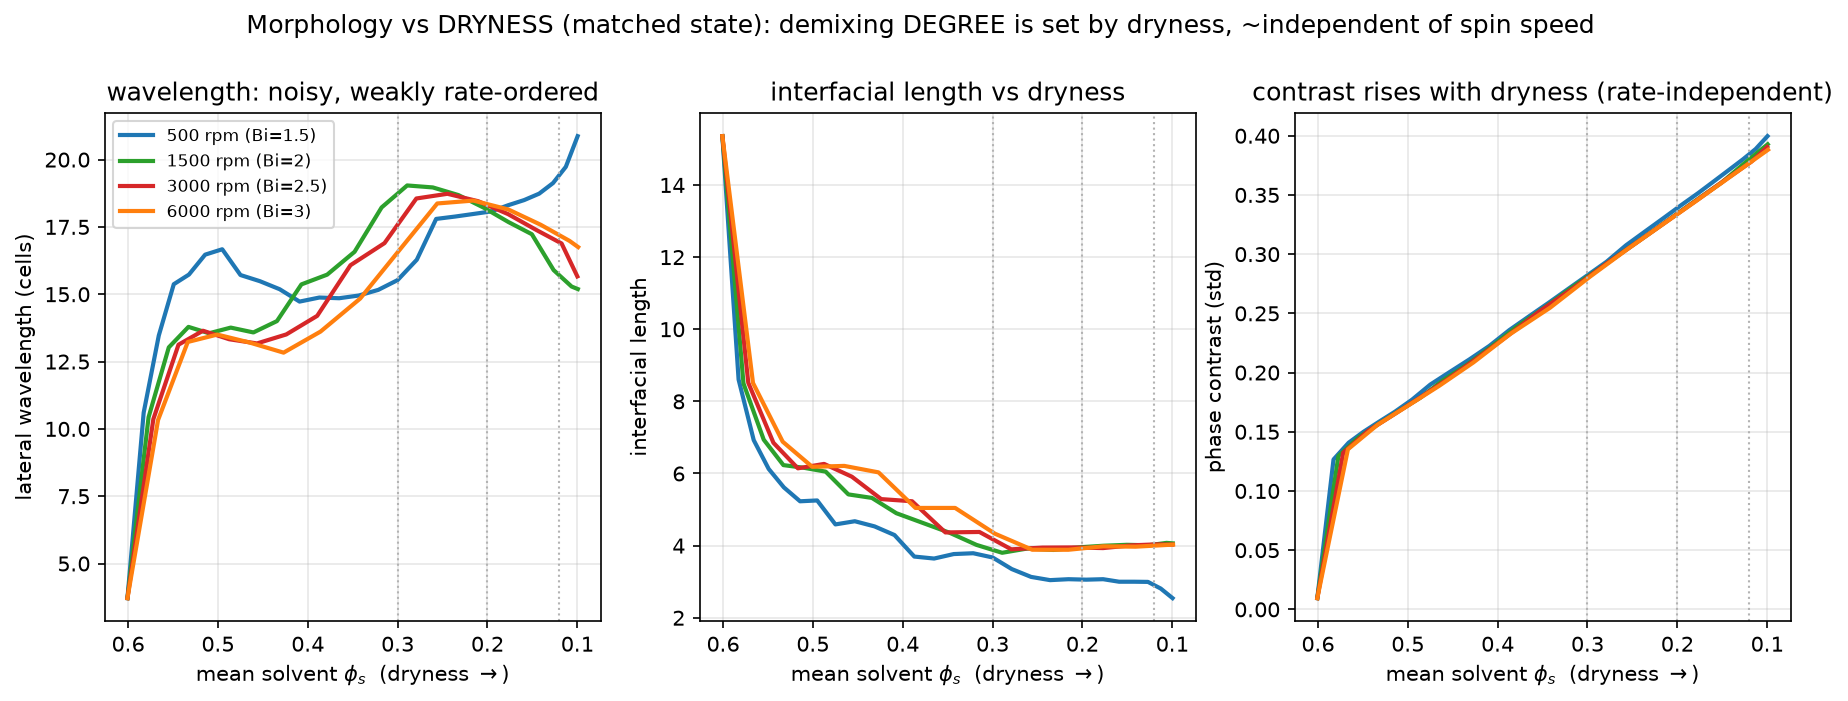
\includegraphics[width=\linewidth]{figures/p10_matched.png}
  \caption{Morphology metrics as a continuous function of dryness $\phi_s$
  (the de-confounded axis). Wavelength (left) is Biot-ordered but noisy;
  interfacial length (centre) and phase contrast (right) rise cleanly with
  dryness and are nearly independent of spin speed at matched $\phi_s$.}
  \label{fig:p10matched}
\end{figure}

% --- generated by gen_figures.py ---
\begin{figure}[h]\centering
  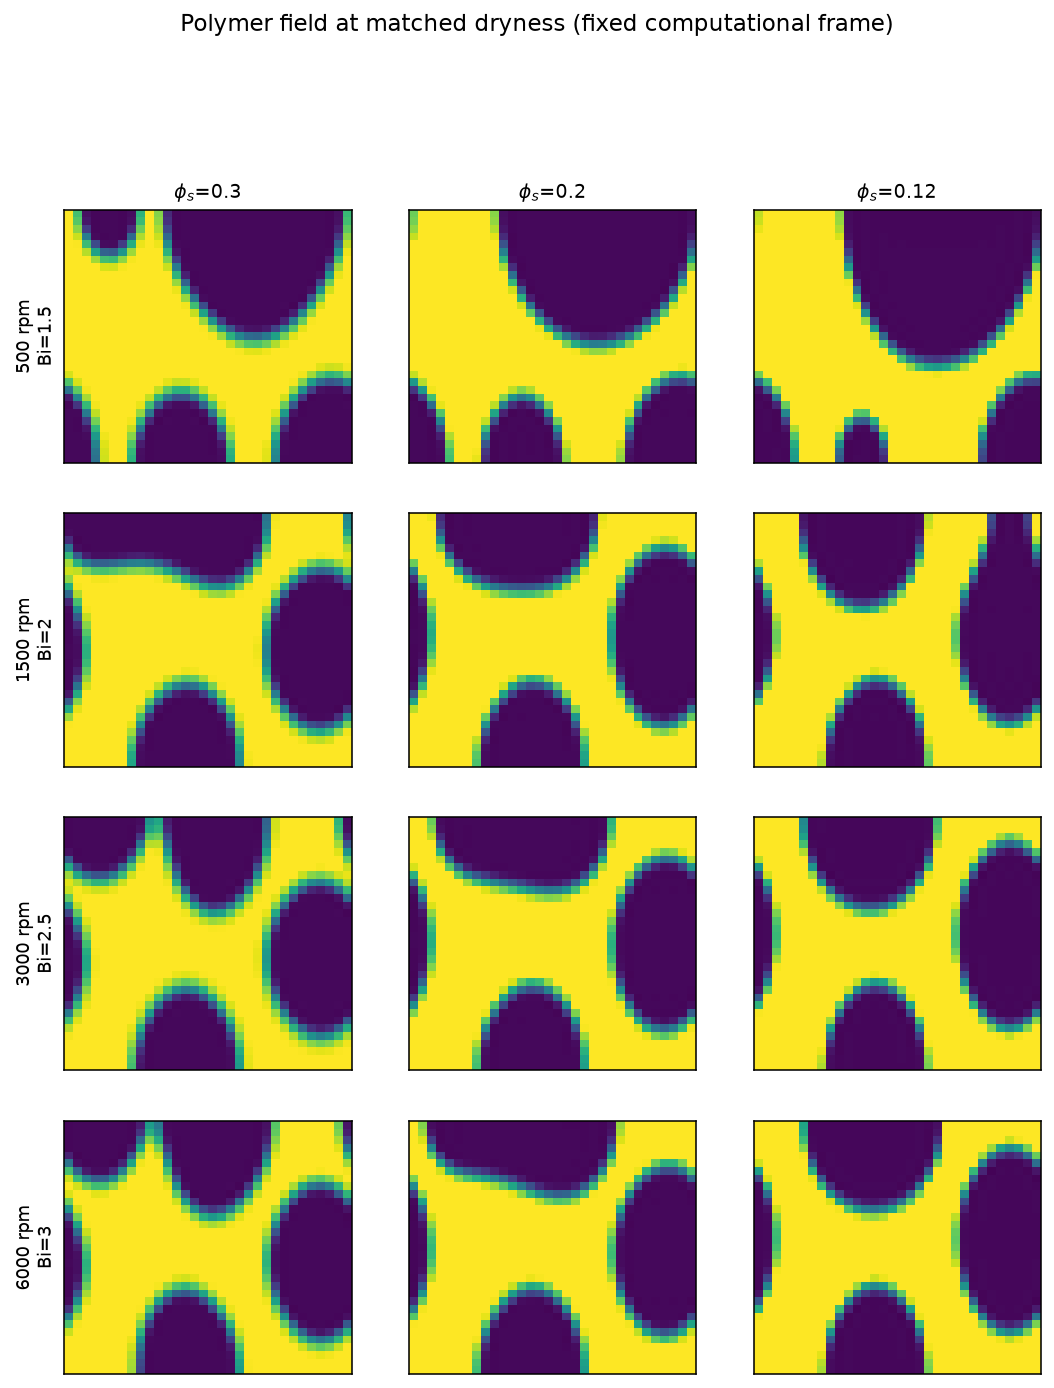
\includegraphics[width=0.85\linewidth]{figures/p10_morphology.png}
  \caption{Polymer field at the matched dryness levels for each ladder rung
  (fixed computational frame). The pattern coarsens/sharpens with dryness far
  more than it changes with spin speed.}
  \label{fig:p10morph}
\end{figure}

\section{Mesh and time convergence}

A reference case is only worth maintaining if its conclusions survive
refinement. The harness repeats one ladder rung on a finer mesh and at smaller
time steps and reports the matched-dryness metrics in mesh-independent form ---
the wavelength as a fraction of the box width, and the phase contrast.
Fig.~\ref{fig:p10conv} shows the demixing-degree conclusion is robust: the
phase contrast changes by only $\PtenMeshDContrast\%$ between the coarse and
fine mesh and by $\PtenTimeDContrast\%$ between the largest and smallest time
step (the box-fraction wavelength moves $\PtenMeshDWL\%$ under mesh
refinement, consistent with its noisier character).

% --- generated by gen_figures.py ---
\begin{figure}[h]\centering
  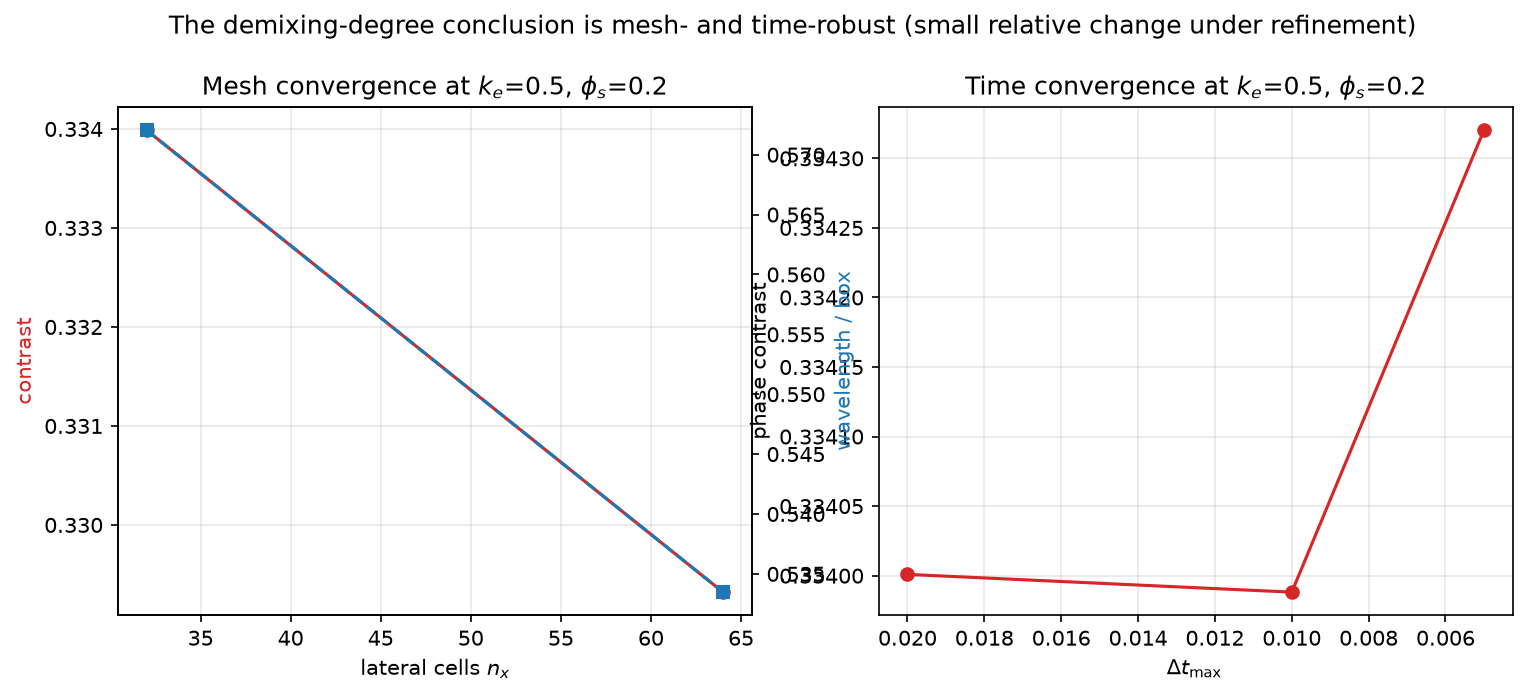
\includegraphics[width=\linewidth]{figures/p10_convergence.png}
  \caption{Mesh (left) and time (right) convergence of the matched-state
  metrics at one ladder rung. The phase contrast --- the robust conclusion ---
  is nearly flat under refinement.}
  \label{fig:p10conv}
\end{figure}

\begin{keybox}
\textbf{A conservation caveat, stated honestly.} With a large polymer
$N=\PtenNpoly$ the polymer segregates into a sharp demixed surface layer that
the $32\times32$ reference mesh only partly resolves, so the per-solute
moving-frame balance for the polymer is $\PtenBalP$ (relative) --- looser than
the fullerene's machine-precision $\PtenBalF$ --- and it tightens as the mesh
refines. The fullerene conservation is the hard, resolution-robust gate; the
polymer residual is reported and tracked, not hidden.
\end{keybox}

\section{Parameter-uncertainty sensitivity}

The recorded $\chi_{pf}$ carries an order-of-magnitude uncertainty, so a robust
conclusion must survive changing it by a factor of a few. The harness sweeps
$\chi_{pf}$ across that band at a fixed rung and dryness (Fig.~\ref{fig:p10sens}).
The demixing DEGREE tracks $\chi_{pf}$ cleanly and monotonically
(monotone: \PtenSensMonotone; contrast spans $\PtenSensSpan\%$ across the band),
exactly as Flory--Huggins predicts --- a stronger enthalpic penalty demixes
harder. The wavelength, by contrast, stays noisy and only weakly
$\chi$-dependent.

% --- generated by gen_figures.py ---
\begin{figure}[h]\centering
  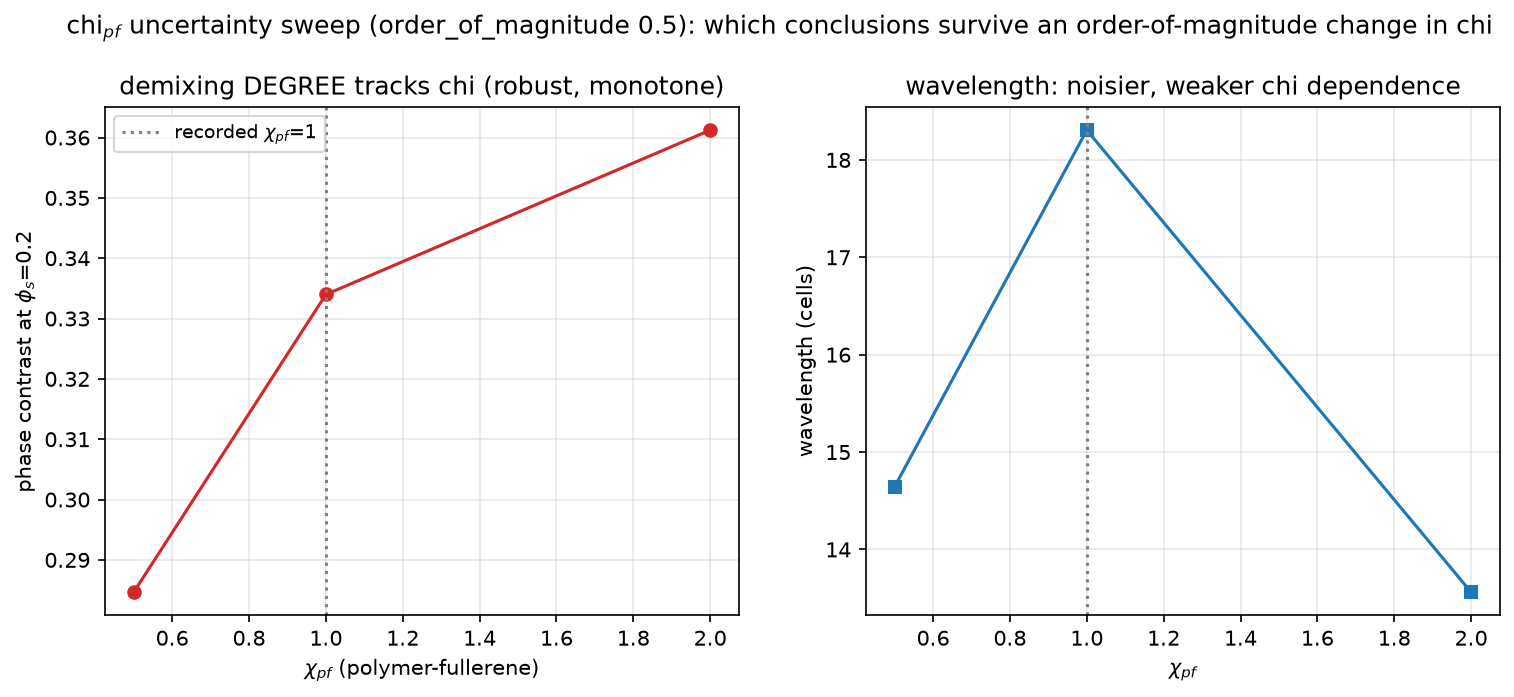
\includegraphics[width=\linewidth]{figures/p10_sensitivity.png}
  \caption{Sensitivity to the order-of-magnitude $\chi_{pf}$ uncertainty. The
  demixing degree (left) is a robust, monotone function of $\chi_{pf}$; the
  wavelength (right) is not a reliable discriminator at this scale.}
  \label{fig:p10sens}
\end{figure}

\section{The robustness verdict}

\begin{keybox}
\textbf{Which conclusions are robust?}
\begin{itemize}[nosep]
\item \textbf{Robust} (survives mesh + time refinement and the $\chi_{pf}$
  uncertainty): the DEGREE of demixing (phase contrast) is set by DRYNESS, rises
  monotonically as the film dries, is nearly rate-independent at matched
  $\phi_s$, and increases monotonically with $\chi_{pf}$. Morphology collapses
  onto the Biot number.
\item \textbf{Not robust at tutorial scale}: the ``faster spin $=$ finer
  morphology'' \emph{wavelength} ordering. With a single seed and only a few
  lateral domains it is noisy, moves under mesh refinement, and is a weak
  function of $\chi_{pf}$. Reproducing it quantitatively needs seed ensembles
  and a larger box --- a research-mode campaign (Chapter~\ref{ch:c9}), not a
  tutorial run.
\end{itemize}
\end{keybox}

This is the scientific habit the capstone is teaching: a real reference case
reports what the data support at the resolution actually run, separates the
robust invariant (demixing degree vs.\ dryness and $\chi$) from the
scale-limited claim (the wavelength ordering), and hands the reader a
tolerance-checked artefact they can re-run and extend.

\section{Explore on your own}

\question{Swap the system to \code{P3HT\_PCBM} in \file{configs/p10.yaml}. Confirm
the honest negative: measure the phase contrast at matched dryness and show it
is far smaller than for \PtenSystem. What does that say about using contrast as
a screening metric for candidate blends?}

\question{Widen the drying-rate window (\code{k\_e\_slow}, \code{k\_e\_fast}) and
re-run. Does a larger Biot span sharpen the ``faster $=$ finer'' wavelength
ordering, or does the noise still dominate at a single seed?}

\question{Run several seeds at one rung and report the wavelength as a mean
$\pm$ spread. How many seeds would you need for the ``faster $=$ finer'' claim
to clear its own error bar? Connect this to the reproducible-campaign machinery
of Chapter~\ref{ch:c9}.}

\question{Push the mesh-convergence rung to level~7 (research mode). Does the
polymer per-solute conservation residual tighten toward the fullerene's
machine-precision value as you predicted from the surface-layer argument?}
